% !TeX root = ../tfg.tex
% !TeX encoding = utf8

\chapter{Experimentos Adicionales: Hiperparámetros}\label{ap:apendiceB}

En este apéndice se presentan dos experimentos relacionados con el uso de diferentes tamaños de lote y tasas de aprendizaje para un modelo que exhibe el doble descenso, con la finalidad de verificar su comportamiento ante distintas configuraciones. Para ello, se empleará la arquitectura $2$NN sobre el subconjunto MNIST[$4000/1000$], al cual se le añadirá un porcentaje variable de ruido, y donde se utilizarán distintas tasas de aprendizaje.
 
\subsection*{Double descent con distinto tamaño de batch}

\begin{figure}[h!]
    \centering
    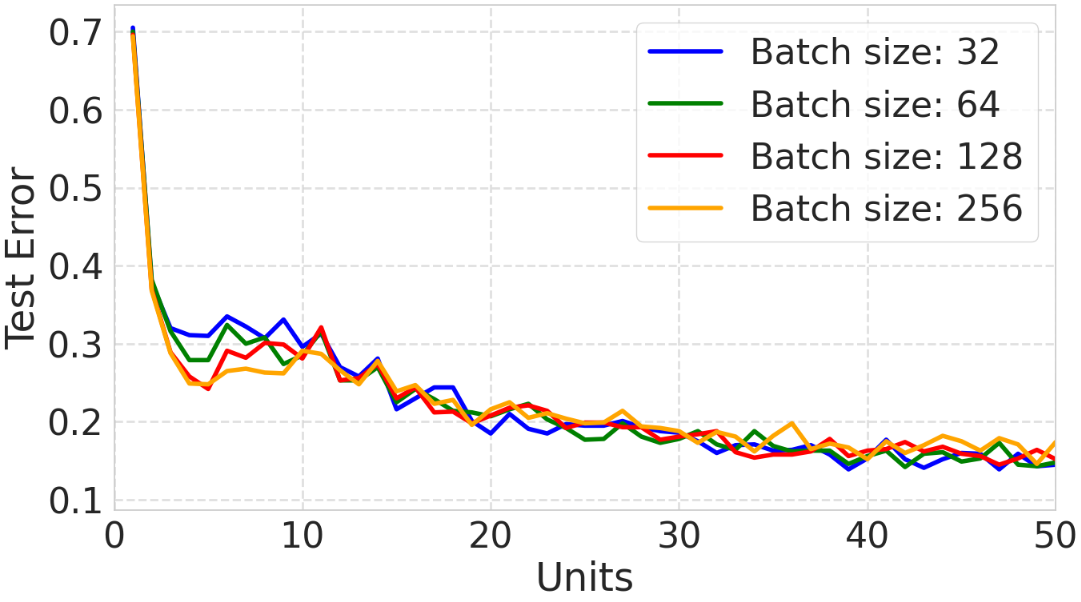
\includegraphics[width=0.65\textwidth]{img/experiments/batch_sizes_ddd.png}
    \caption[Doble descenso para distintos tamaños de lote.]{Error en test respecto a distintas configuraciones de tamaño de batch de la red $2$NN sobre el subconjunto MNIST[$4000/1000$] con $10$\% de ruido añadido.}\label{fig:dddbatchsizes}
\end{figure}

En la Figura~\ref{fig:dddbatchsizes} se observa que, para distintas configuraciones de tamaño de batch, se manifiesta el doble descenso, siendo más notable (sin tantos altibajos en la curva del error) al utilizar tamaños de lote mayores, debido a que se utiliza un mayor número de ejemplos para actualizar los parámetros en cada iteración. Por otro lado, la Tabla~\ref{tab:dddbatchsizes} muestra que, al incrementar el tamaño de batch, el tiempo de entrenamiento disminuye, lo cual es lógico, ya que se procesan un mayor número de ejemplos en cada iteración. Por tanto, considerando ambos resultados, se concluye que utilizar un tamaño de lote elevado ($128$ o $256$) es la opción adecuada para los distintos experimentos a realizar, ya que permite observar el fenómeno de forma más precisa y con menor coste computacional.

\begin{table}[h!]
    \centering
    \begin{tabular}{|c|c|c|c|}
    \hline
    \textbf{Modelo}       & \textbf{Dataset} & \textbf{Batch size} & \textbf{Entrenamiento} \\ 
    \hline
    $2$NN ($1-50$)     & MNIST[$4000/1000 - 10$\% noise]      & $32$      & $15$h $2$min         \\ 
    $2$NN ($1-50$)     & MNIST[$4000/1000 - 10$\% noise]      & $64$      & $11$h $56$min         \\ 
    $2$NN ($1-50$)     & MNIST[$4000/1000 - 10$\% noise]      & $128$      & $11$h $14$min         \\ 
    $2$NN ($1-50$)     & MNIST[$4000/1000 - 10$\% noise]      & $256$      & $10$h $23$min         \\
    \hline
    \end{tabular}
    \caption[Resumen de los experimentos realizados para el doble descenso con distinto tamaño de lote.]{Resumen de los experimentos realizados para el doble descenso con distinto tamaño de lote.}\label{tab:dddbatchsizes}
\end{table}

\subsection*{Double descent con distinto learning rate}

\begin{figure}[h!]
    \centering
    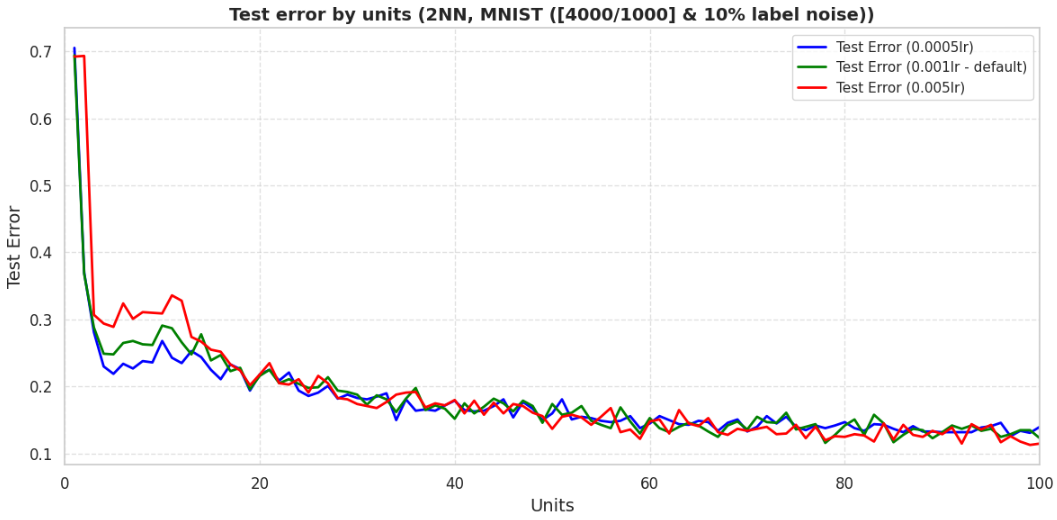
\includegraphics[width=0.65\textwidth]{img/experiments/learning_rates_ddd.png}
    \caption[Doble descenso para distinto \textit{learning rate}.]{Error en test respecto a distintas configuraciones de \textit{learning rate} obtenido por la red $2$NN sobre el subconjunto MNIST[$4000/1000$] con $10$\% de ruido añadido.}\label{fig:difflr}
\end{figure}

En la Figura~\ref{fig:difflr} podemos observar cómo se manifiesta el doble descenso para distintas configuraciones de la tasa de aprendizaje. En particular, el pico del error de test se hace más pronunciado a medida que la tasa de aprendizaje aumenta, dado que para un \textit{learning rate} igual a $5 \times 10^{-4}$, el máximo error en test es mayor que para el valor por defecto de la tasa de aprendizaje ($10^{-4}$) del optimizador Adam, y este, a su vez, es mayor que el máximo valor que proporciona la mínima tasa de aprendizaje utilizada ($5 \times 10^{-5}$).

En conclusión, esto nos indica que, si un modelo presenta el \textit{Deep Double Descent}, no es necesario preocuparse en exceso por ajustar de manera precisa la tasa de aprendizaje, puesto que, dentro de ciertos rangos de valores de este hiperparámetro, el comportamiento característico del doble descenso se mantiene, lo que indica que el uso por defecto de la tasa de aprendizaje resulta ser suficiente.

Finalmente, para concluir esta subsección se muestra en la Tabla~\ref{tab:difflr} un resumen de los experimentos realizados junto con sus respectivos tiempos de entrenamiento.

\begin{table}[h!]
    \centering
    \begin{tabular}{|c|c|c|c|}
    \hline
    \textbf{Modelo}       & \textbf{Dataset} & \textbf{Tasa aprendizaje} & \textbf{Entrenamiento} \\ 
    \hline
    $2$NN ($1-100$)     & MNIST[$4000/1000 - 10$\% noise]      & $0.005$      & $23$h $53$min         \\ 
    $2$NN ($1-100$)     & MNIST[$4000/1000 - 10$\% noise]      & $0.001$ (\textit{default})      & $26$h $50$min     \\ 
    $2$NN ($1-100$)     & MNIST[$4000/1000 - 10$\% noise]      & $0.0005$      & $27$h $32$min         \\ 
    \hline
    \end{tabular}
    \caption[Resumen de los experimentos realizados para el doble descenso con distinto \textit{learning rate}.]{Resumen de los experimentos realizados para el doble descenso con distinto \textit{learning rate}.}\label{tab:difflr}
\end{table}

\endinput
%------------------------------------------------------------------------------------
% FIN DEL APÉNDICE. 
%------------------------------------------------------------------------------------
